\subsubsection{Customer Reporting}
			To accompany this diagram, read the Scenario \hyperref[sec:CustomerReportingScenario]{S.8}.

				\begin{table}[htpb]
					\centering
					\label{tab:CustomerReportingDiagramTable}
					\begin{tabularx}{\textwidth}{lp{9cm}}
						\hline
						\hline
							\textbf{Subject}
						& 
							\textbf{Description}\\
						\hline
							Actors	       &  Taxi Driver, myTaxiService Mobile Application, myTaxiService Server\\
						\hline
							Preconditions  &  Taxi Driver must be logged in.\\
						\hline
							Execution      &  1.~Taxi Driver opens the myTaxiService Mobile Application.\\
										   &  2.~Taxi Driver receives a ride request notification from the Application.\\
										   &  3.~Taxi Driver accepts the ride request.\\
										   &  4.~Taxi Driver goes to the meeting location and the Customer is not there.\\
										   &  5.~Taxi Driver ends the ride reporting an abuse.\\
						\hline
							Postconditions &  The ride is set to 'ended' and the Customer is reported.\\
						\hline
							Exceptions     &  1.~The Taxi Driver disconnects before reporting.\\
									
						\hline
						\hline
					\end{tabularx}
				\end{table}
				
				\begin{figure}[H]
					\centering
					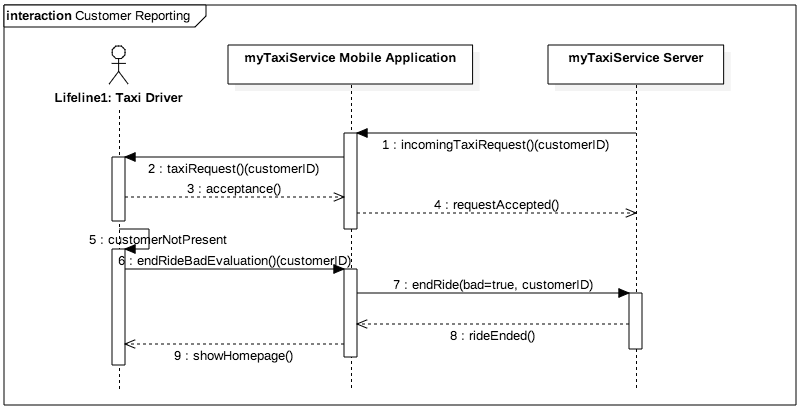
\includegraphics[width=\textwidth, scale=0.5]{IMG/InteractionDiagrams/CustomerReporting.png}
					\caption{Customer Reporting Interaction Diagram}\label{sec:FigureCustomerReporting}
				\end{figure}